\newSec[HWCOEX]{COEX Drohne}{2}

Bei dem für die \DHBW\ neu angeschafften \Quad\ handelt es sich um das Modell \Clover\ des Unternehmens \textit{Copter Express} (\COEX).

Das Modell \Clover\ wurde vom Hersteller zur Ausbildung und Forschung an \Quad[n] entwickelt. Das Modell besitzt einen Rahmen, welche die Rotoren bei Kollisionen schützten soll.




Interner Flight Controller, ROS Kommunikation via Pie 4.




Probleme bei Inbetriebnahme - Beispielprogramm des Herstellers bringt nicht das erwartete Ergebnis.




\newSec[Control]{Control Stack}{3}
Als \textit{Flight Controller} wird das Modell \textit{PX4 Racer} genutzt. Die Firmware, sowie weitere Software zur Interaktion mit der Drohne \Clover\ werden von \textit{Dronecode Foundation} bereitgestellt.

Die Anbindung an \ROS wird durch einen \Pie\ realisiert. Hierbei wird der On-Board Computer als \textit{roscore} genutzt.


\newSec{Funkfernsteuerung}{3}
s-Bus ??





\newSec{Sensorik}{3}

\missing[EIn bisschen Einleitung.]


\begin{itemize}
\item Gyroskop
\item Laser-Abstandsmessung zum Boden
\item GPS
\item Bodenkamera
\end{itemize}










\newSec[Build]{Aufbau des Bausatzes}{3}





\newSec{Aufbau}{4}

\missing[Bilder vom Aufbau]





\begin{figure}[ht!]
\vspace{0.25cm}
\begin{center}
\fbox{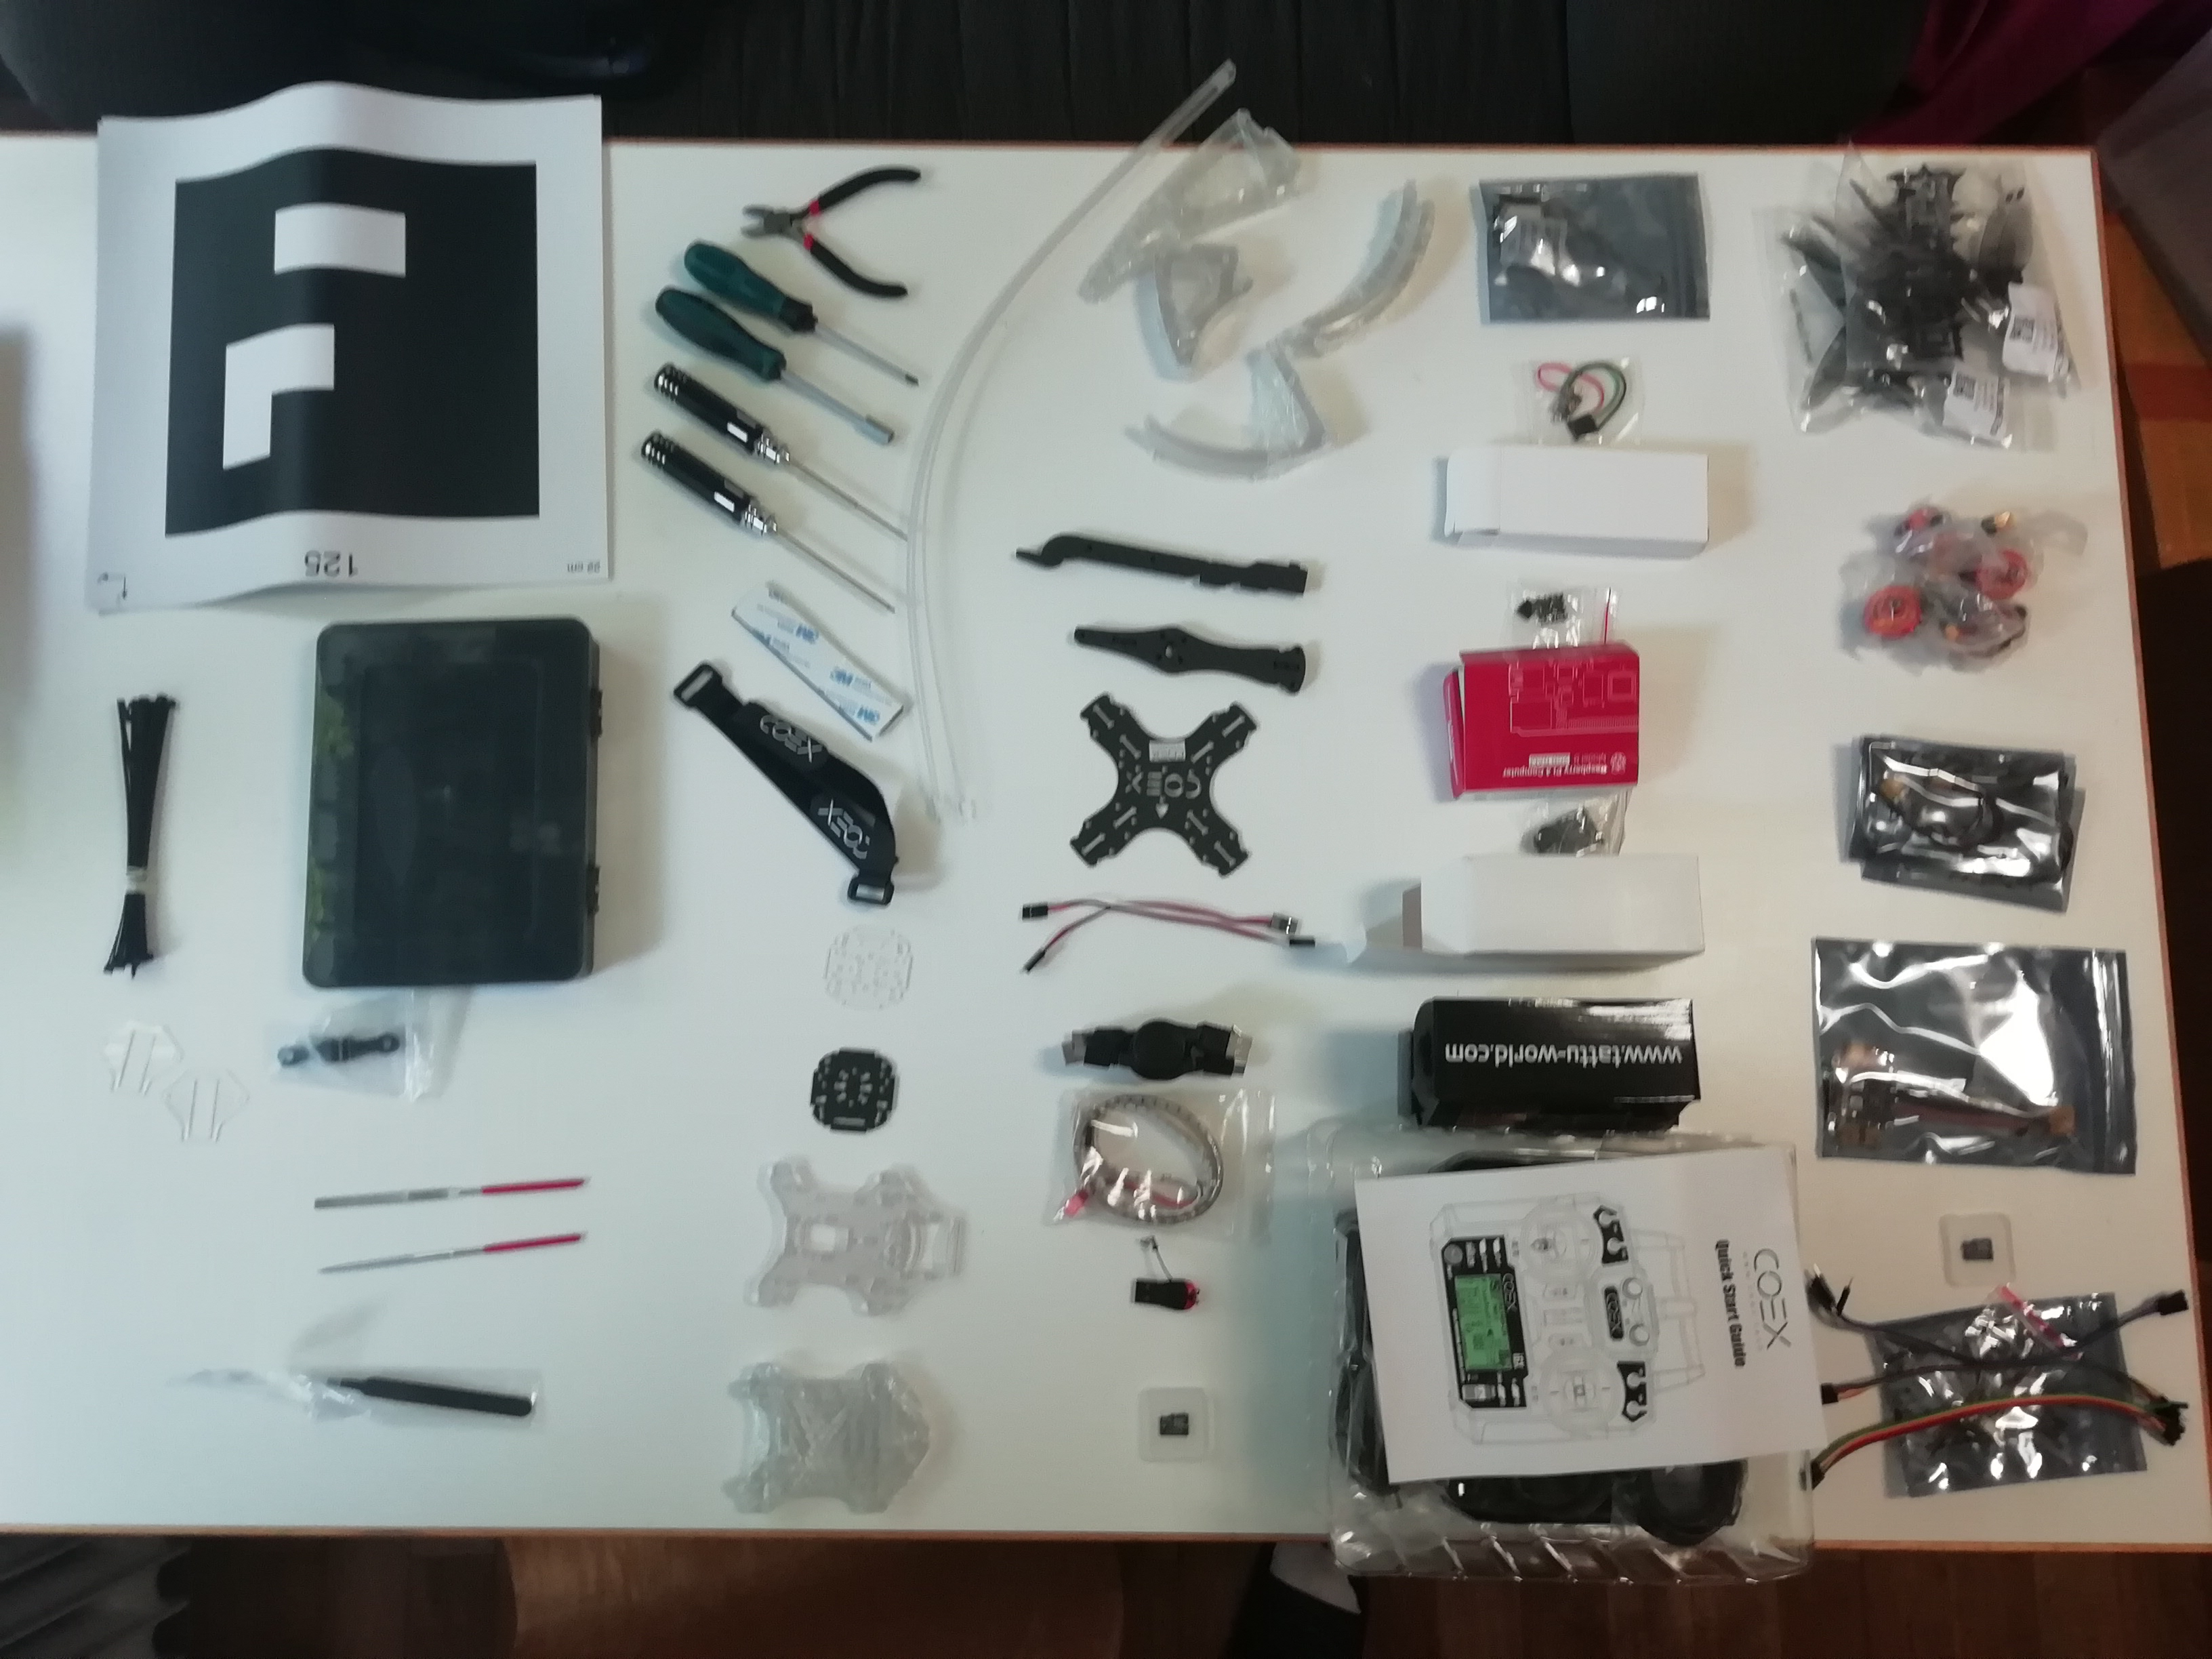
\includegraphics[width=7.5cm]{Pictures/Aufbau1.jpg}}\hfill
\fbox{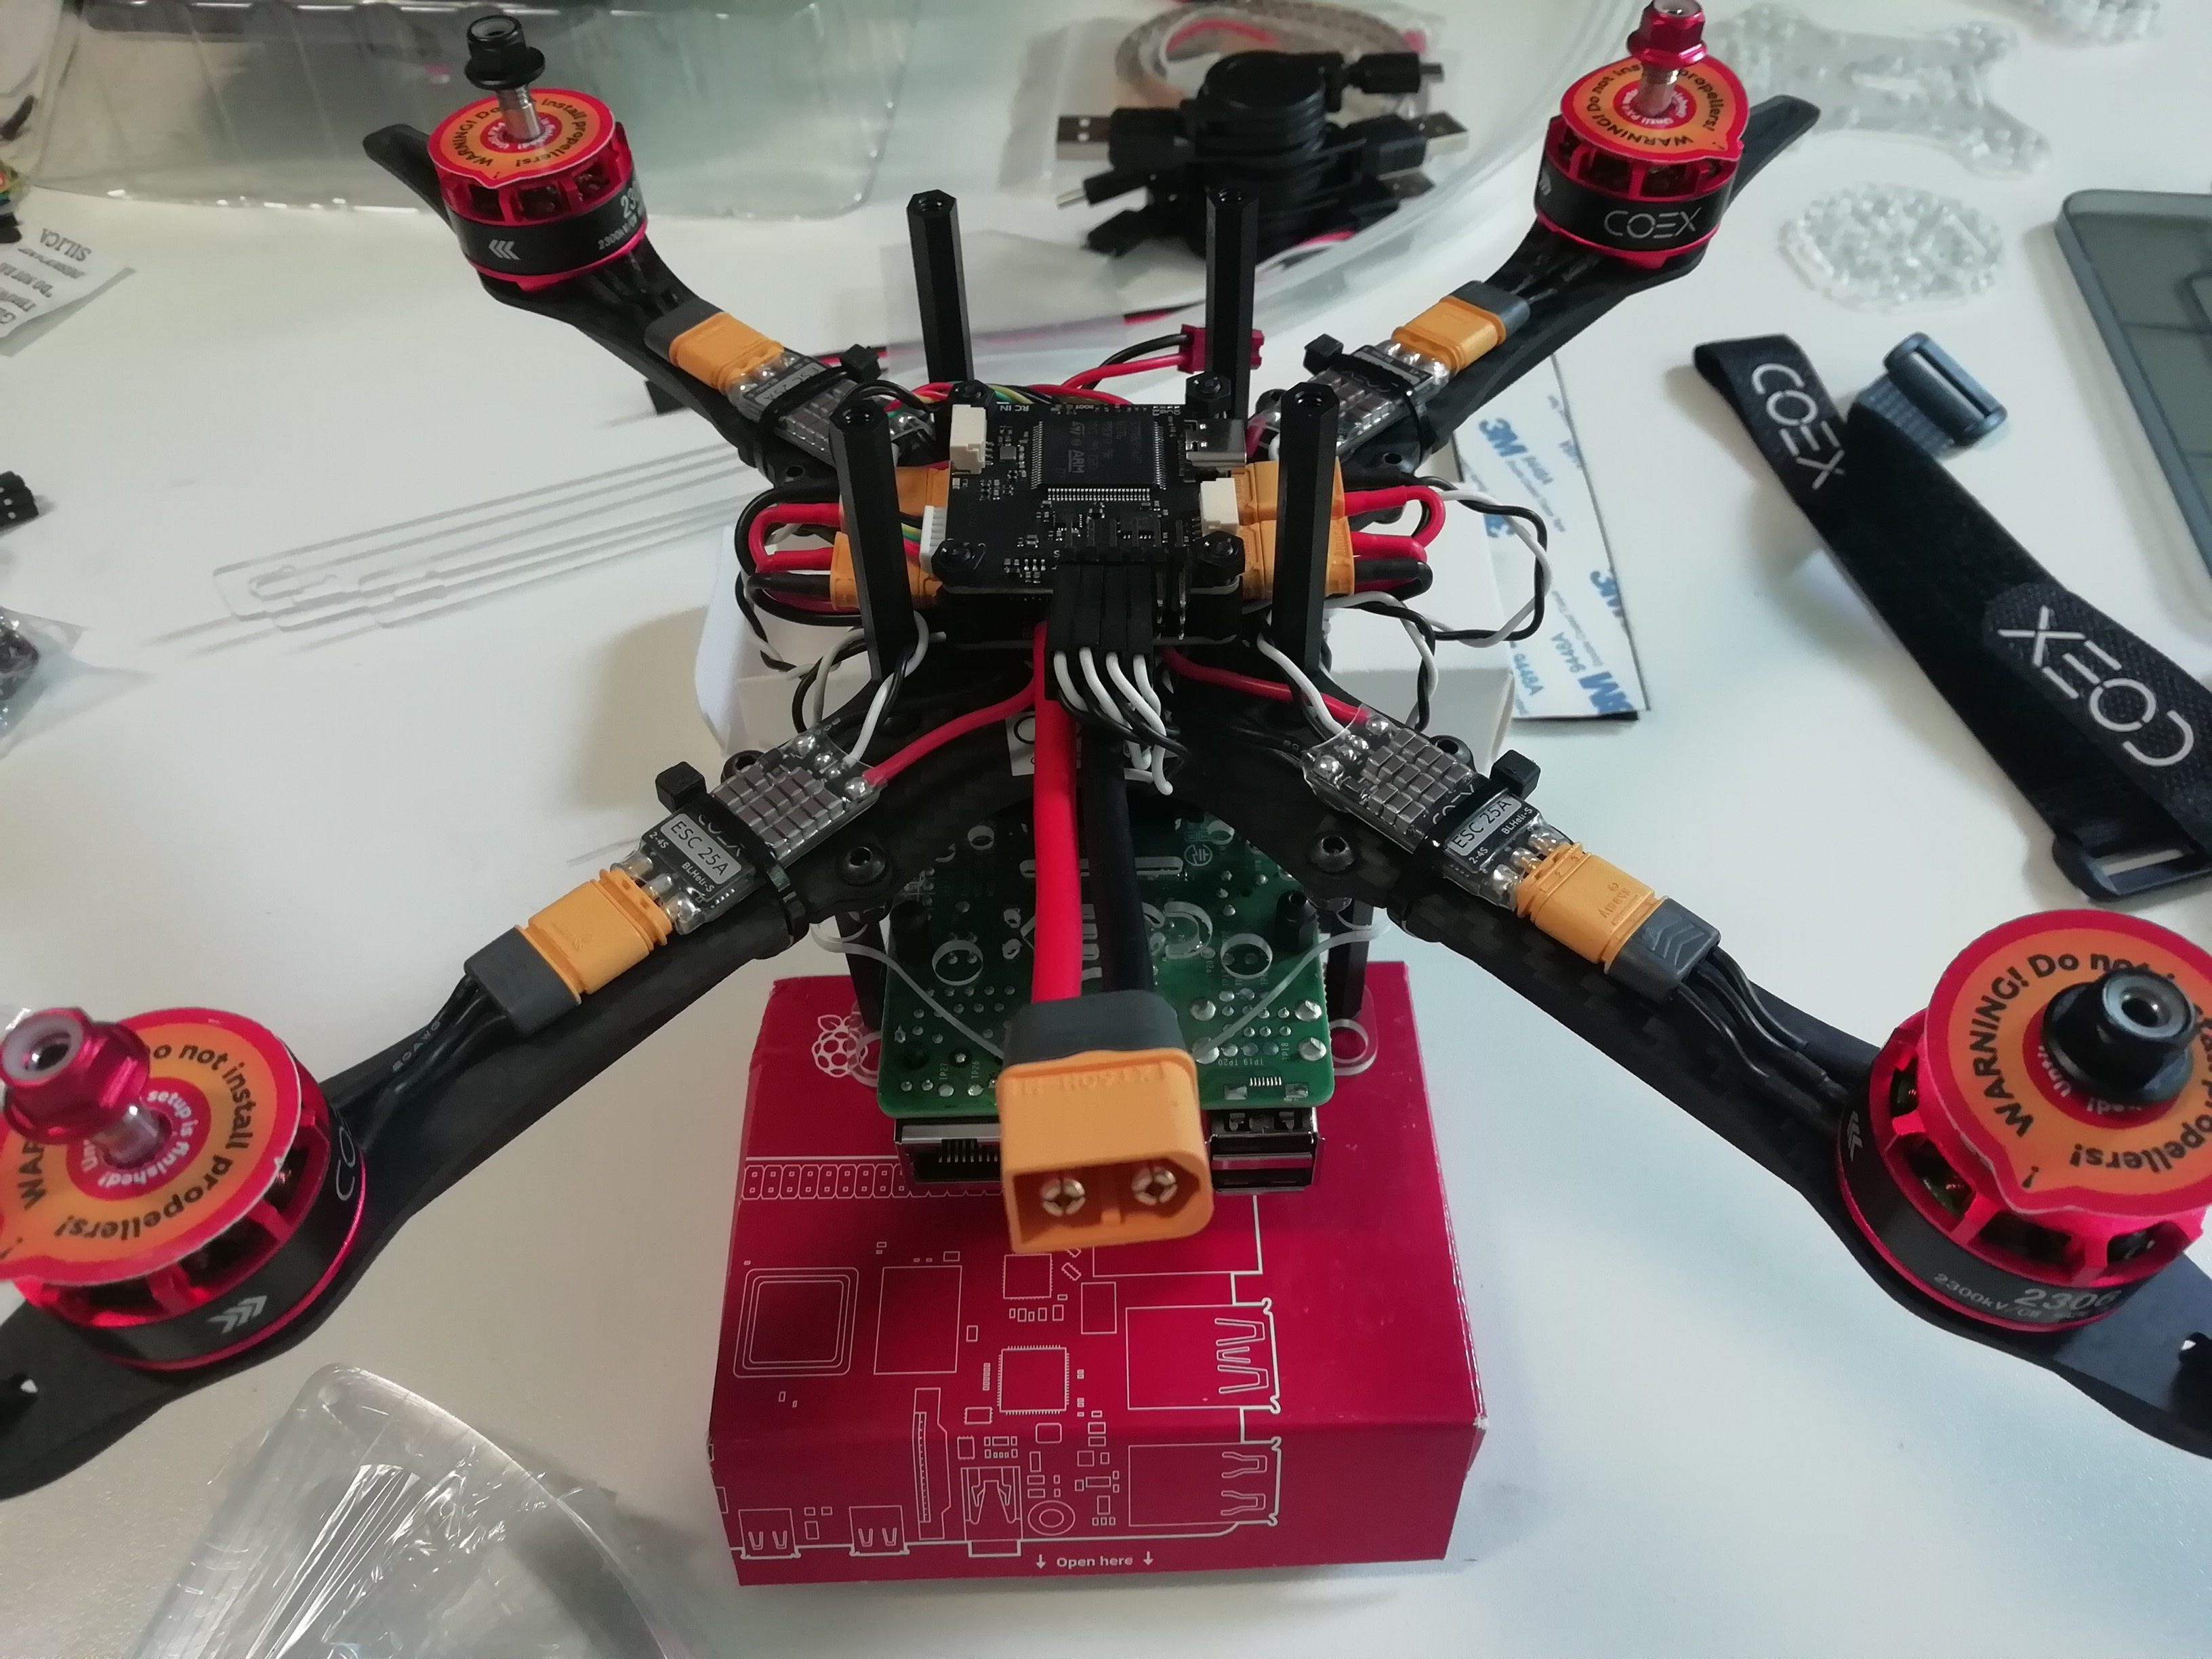
\includegraphics[width=7.5cm]{Pictures/Aufbau2.jpg}}
\fbox{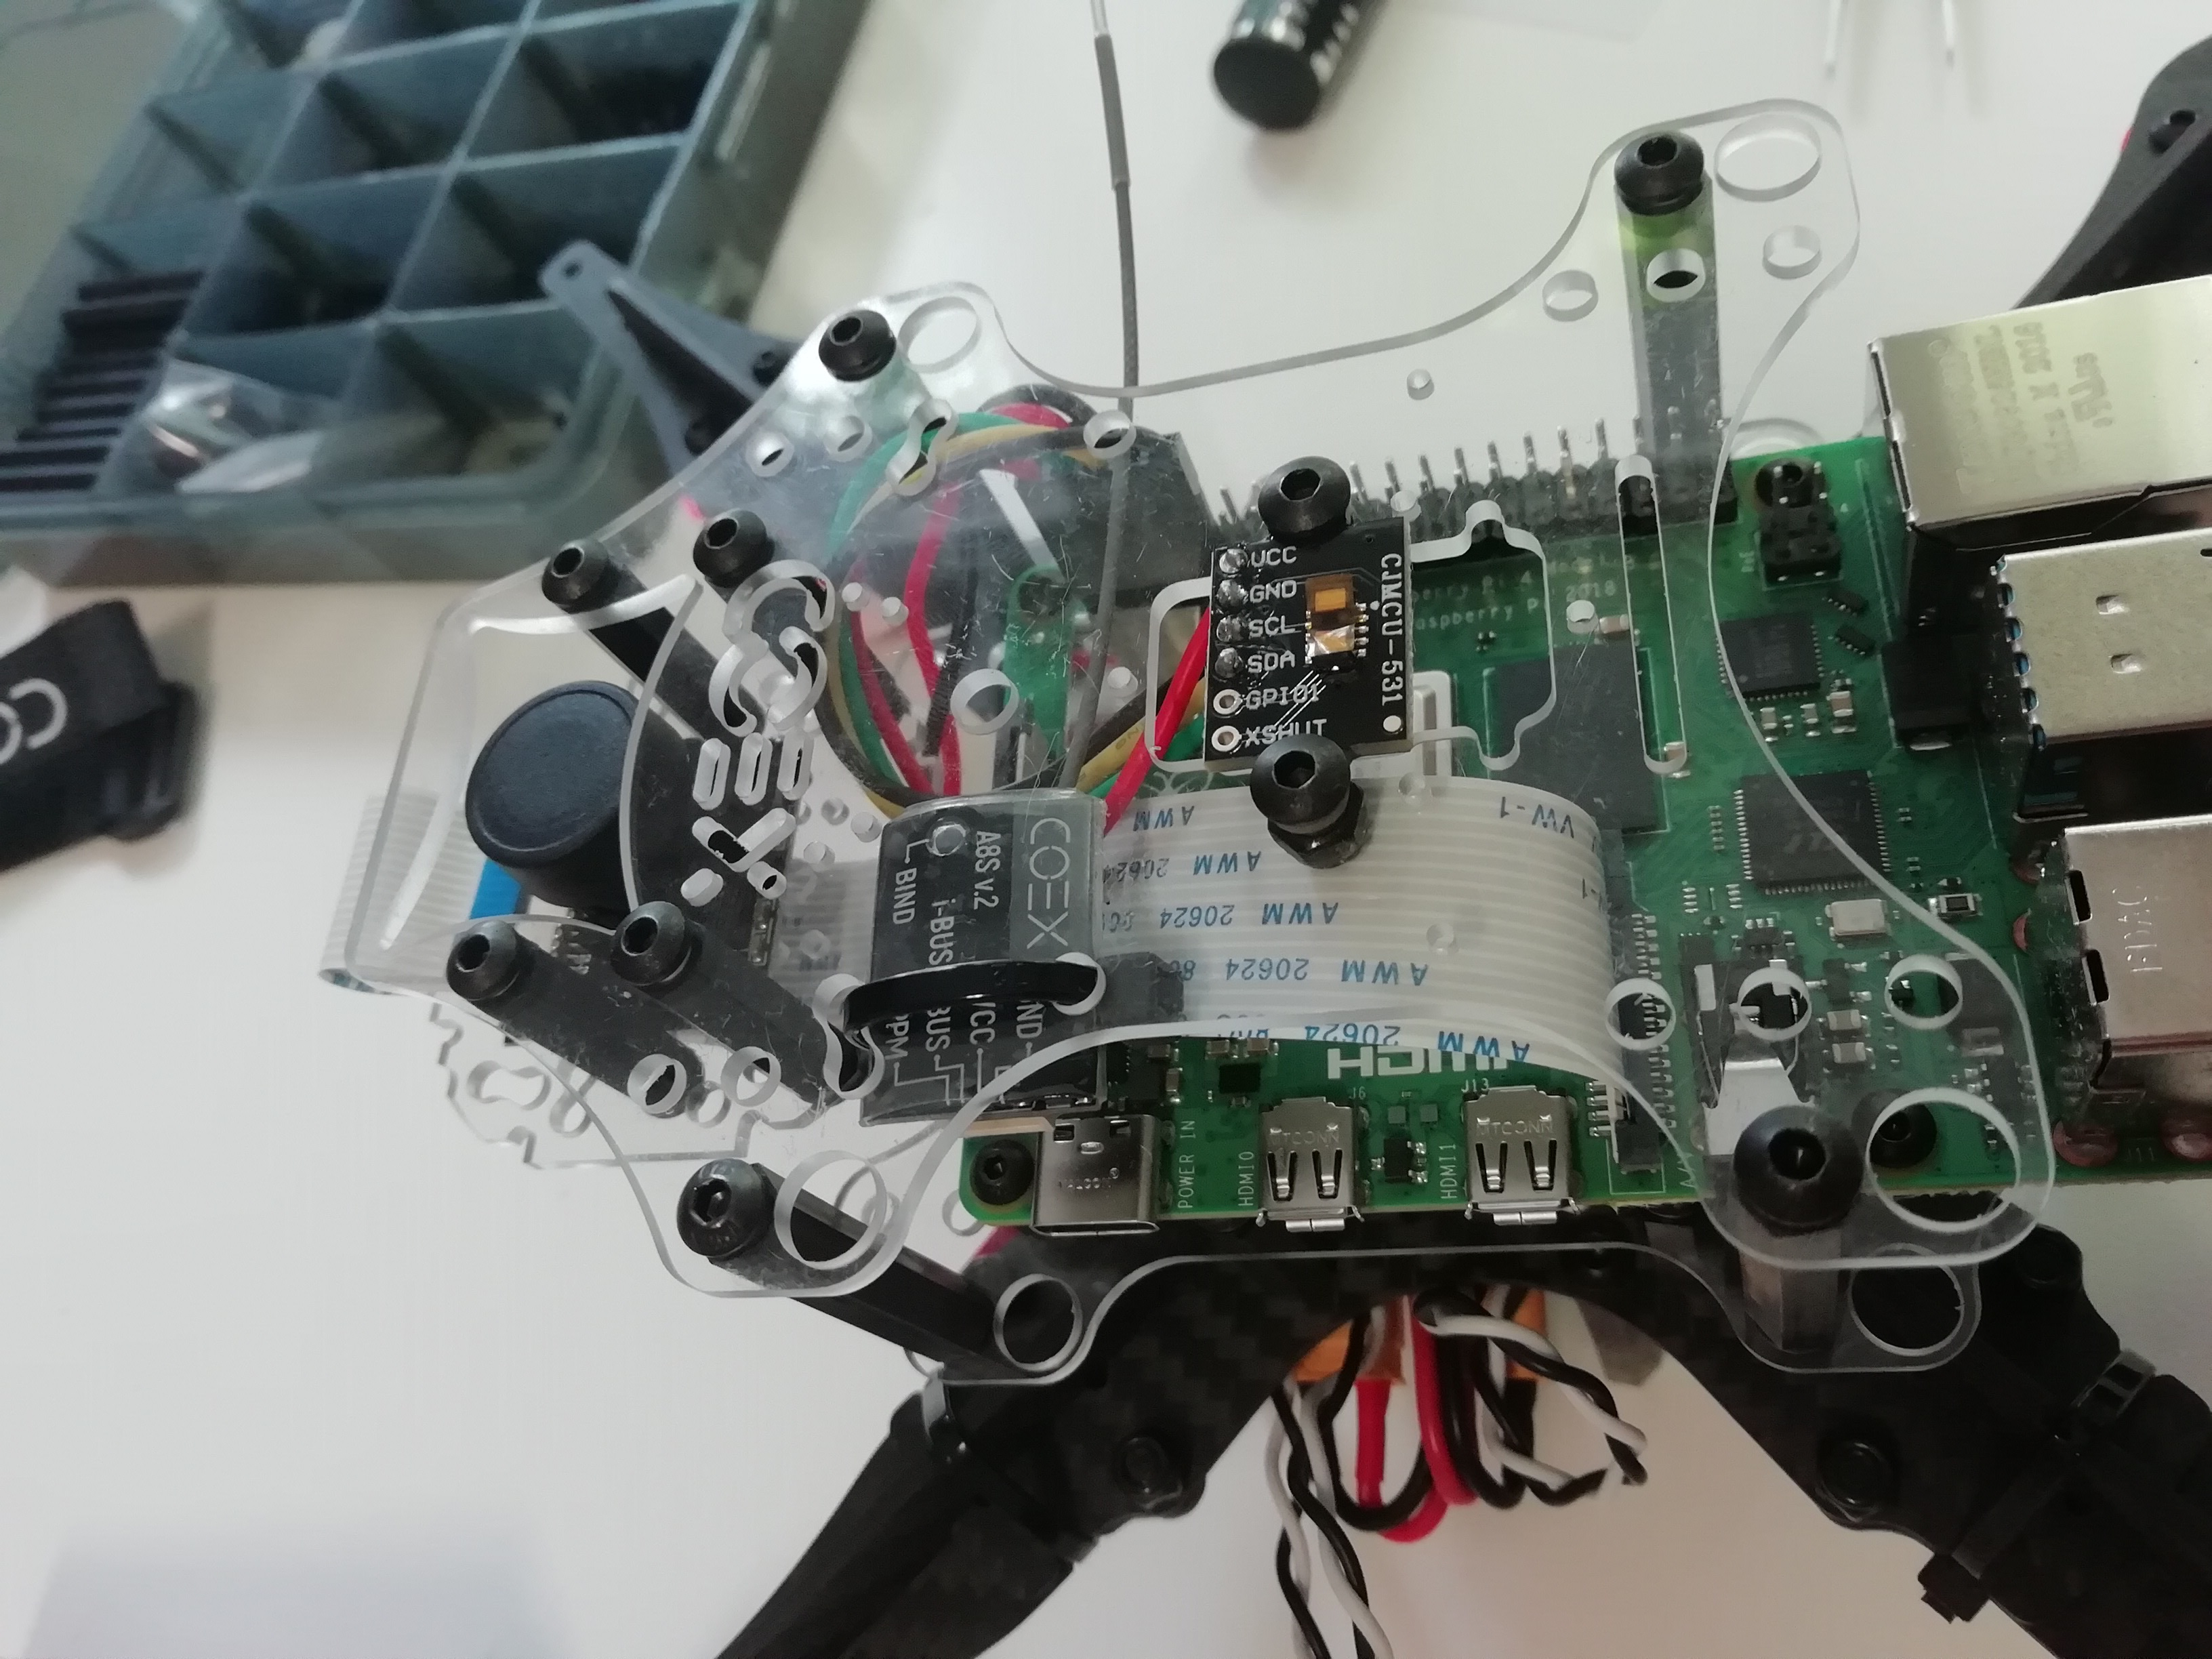
\includegraphics[width=7.5cm]{Pictures/Aufbau3.jpg}}\hfill
\fbox{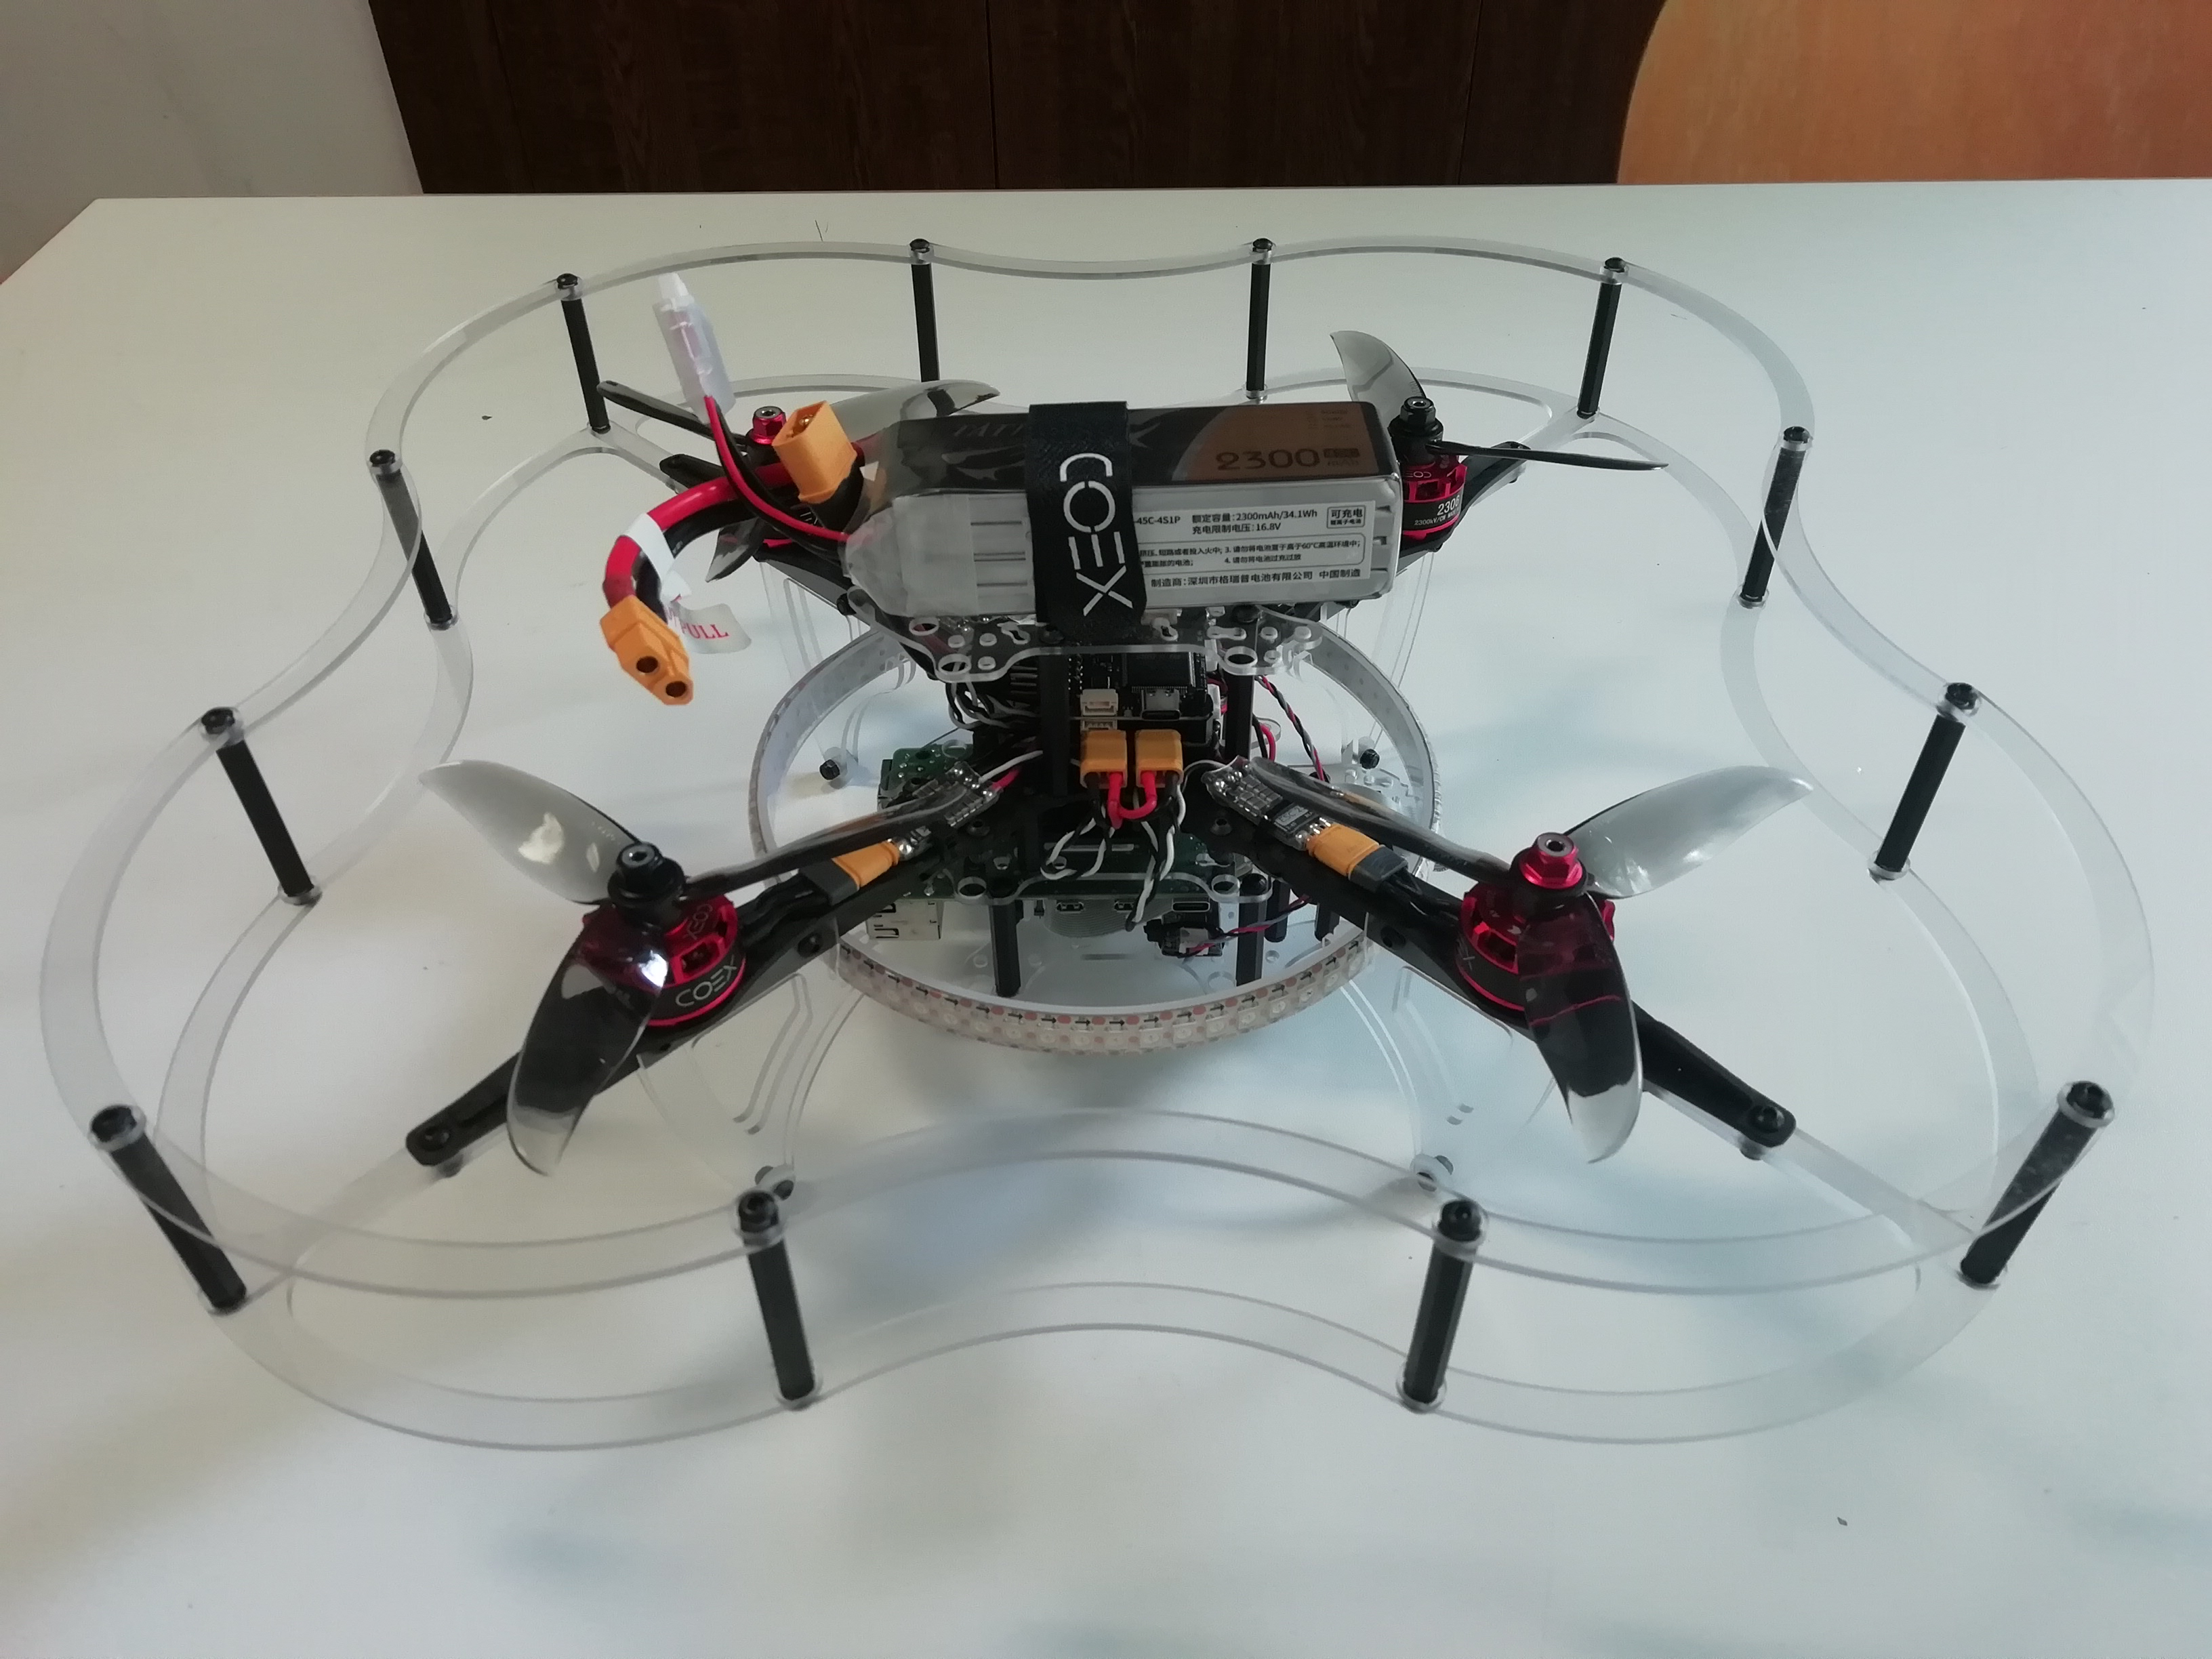
\includegraphics[width=7.5cm]{Pictures/Aufbau4.jpg}}
\caption{Aufbau des Bausatzes für die Drohne \Clover}
\label{fig:coexBuild}
\end{center}

\vspace{0.25cm}
\refImgShort{fig:coexBuild} zeigt etappenweise den Aufbau des Bausatzes für die Drohne \Clover. Hierbei ist die zeitliche Anordnung in der Collage zeilenweise zu interpretieren.
\end{figure}







\newSec[Build]{Inbetriebnahme}{3}


\newSec{Konfiguration des Flight Controllers}{4}



\newSec{Testflug}{4}



\comp{coexExample}
\missing[Verweis auf Example Code]













\newSec[Build]{Mögliche Lösung der Aufgabenstellung}{3}



\newSec[COEXPkg]{COEX-Package}{4}
Für die Interaktion mit der \COEX-Drohne wurden diverse Klassen erstellt, um einzelne Aspekte der Interaktion mit der Drohne umsetzen zu können (siehe \refCap{ImplPlugCOEX}).

Nach dem Wechsel auf die andere Drohne wurde die Aktualisierung dieses Package nicht weiter verfolgt. Sofern eine Einbindung der \COEX-Drohne in die Ergebnisse dieser \Arbeit\ durchgeführt werden soll, müss dieses Package entsprechend angepasst werden.



\newSec[COEXPkgTopic]{geeignete Topics}{4}

Mit dem \rTopic{blablub} \missing\ kann eine Regelung in der XY-Ebene umgesetzt werden. Die Höhenregelung kann mit set\_attitude/thrust eingeführt werden.
Somit wäre der Versuch für nachfolgende Studierende sehr viel sicherer und so.


\missing\


Das \rTopic{/mavros/rc/override} erlaubt das Überschreiben der RC-Kanäle, somit können einzele Eingaben durch den Controller übernommen werden.
\missing\





\newSec[CoexLiteratur]{hilfreiche Literatur}{4}
Nachfolgend sollen Internetseiten genannt werden, welche die Einarbeitung in den Umgang mit der \COEX-Drohne vereinfachen können.

\begin{itemize}
\item https://clover.coex.tech/en/wifi.html

\item https://clover.coex.tech/en/simple\_offboard.html
\item https://docs.px4.io/master/en/ros/mavros\_offboard.html
\item https://docs.px4.io/master/en/flight\_modes/offboard.html

\item https://mavlink.io/en/services/manual\_control.html
\item http://wiki.ros.org/mavros\#mavros.2FPlugins.manual\_control

\item https://mavlink.io/en/messages/common.html\#SET\_POSITION\_TARGET\_LOCAL\_NED
\end{itemize}

Spezifische Verweise sind im Quellcode des \COEX-Package hinterlegt.



\newSec[COEXTrouble]{Troubleshooting}{3}



\missing[Achtung: der Regler VRA muss so eingestellt sein, dass "manual Flight" verfügbar ist. Andersfalls ist ein Start der Drohne nicht möglich.]





\newSec{Platinenfehler}{4}

\missing[Hier anmerken, dass das Problem bisher nicht behoben wurde => Wirkt sich nur auf LED-Streifen aus.]





\newSec{Bus-System des RC Empfängers}{4}
\missing[RC-Empfänger gibt per default i-Bus aus, PX4 erwartet s-Bus.]

\missing[Bild von Oszilloskop]


\texttt{Lösung}\\
\missing[i-Bus und s-Bus werden durch Halten des Knopfens getauscht. Verweis auf Homepage angeben?]





\newSec[TopicTroubleRCOverMD5]{md5-Sum des Topics OverrideRCIn}{4}
Nach erfolgreicher Kompilierung wird nachfolgender Laufzeitfehler ausgegeben, wenn sich ein \CodeClass{ros::Subscriber} oder ein \CodeClass{ros::Publisher} auf das \rTopic{/mavros/rc/override} anmeldet:\\
\textcolor{red}{[ERROR] [1643616625.226584828]: Client [/mavros] wants topic /mavros/rc/override \\to have datatype/md5sum [mavros\_msgs/OverrideRCIn/73b27a463a40a3eda1f9fbb1fc86d6f3], but our version has [mavros\_msgs/OverrideRCIn/fd1e1c08fa504ec32737c41f45223398]. Dropping connection.}

\texttt{Lösung}\\
Definition von \\\CodeMeth{struct MD5Sum<::mavros\_msgs::OverrideRCIn\_<ContainerAllocator>>} \\aus 

\begin{lstlisting}[style=Style_Bash, caption=Befehl zum Öffnen des \textit{OverrideRCIn}-Headers]
sudo nano /opt/ros/noetic/include/mavros_msgs/OverrideRCIn.h
\end{lstlisting}

\begin{lstlisting}[style=Style_CPP, numbers=none, caption=Definition des Struct \CodeStruct{MD5Sum} für das Template \textit{OverrideRCIn}]
template<class ContainerAllocator>
struct MD5Sum<::mavros_msgs::OverrideRCIn_<ContainerAllocator>>
{
	static const char* value()
	{
		return "73b27a463a40a3eda1f9fbb1fc86d6f3";
	}

	static const char* value(const ::mavros_msgs::OverrideRCIn_<ContainerAllocator>&)
	{
		return value();
	}
	
	static const uint64_t static_value1 = 0x73b27a463a40a3edULL;
	static const uint64_t static_value2 = 0xa1f9fbb1fc86d6f3ULL;
};
\end{lstlisting}

von dem \Pie\ kopieren und in der Definition des lokalen \ROS\ \textit{\mbox{OverrideRCIn}}-Headers ersetzen.
Ein Versuch, den \Pie\ einem Update zu unterziehen, ist fehlgeschlagen. Somit ist eine unmittelbare Synchronisation der Nachrichten-Typen aufwändig.


